%Phần thiết đặt trang
\documentclass[12pt,a4paper]{article}
\usepackage[LGRgreek]{mathastext}
\usepackage[utf8]{vietnam}
\usepackage{amsfonts}
\usepackage{amsmath}
\usepackage{amssymb}
\usepackage{graphicx}
\usepackage[left=2cm,right=2cm,top=2cm,bottom=2cm]{geometry}
\setlength{\parindent}{0pt}
\usepackage{parskip}
\setlength{\parskip}{0.5em}

%Phần thiết kế khung code nhập liệu
\usepackage{listings}
\usepackage{color}

\definecolor{dkgreen}{rgb}{0,0.6,0}
\definecolor{gray}{rgb}{0.5,0.5,0.5}
\definecolor{mauve}{rgb}{0.58,0,0.82}

\lstset{frame=tb,
  language=C++,
  aboveskip=3mm,
  belowskip=3mm,
  showstringspaces=false,
  columns=flexible,
  basicstyle={\small\ttfamily},
  numbers=left,
  numberstyle=\small\color{gray},
  keywordstyle=\color{blue},
  commentstyle=\color{dkgreen},
  stringstyle=\color{mauve},
  breaklines=true,
  breakatwhitespace=true,
  tabsize=3
}

%Phần chọn font chèn câu lệnh giữa đoạn
\newenvironment{code}{\ttfamily}{\par}
\DeclareTextFontCommand{\chuyencode}{\code}

%Nội dung chính
\begin{document}
%Chỉnh loại tiêu đề chương thành I, II
\renewcommand\thesection{\Roman{section}.}
\renewcommand\thesubsection{\arabic{subsection}.}
\renewcommand\thesubsubsection{\alph{subsubsection}.}
%Mục lục
\tableofcontents

%Chương 1:
\section{Cơ bản về MATLAB}
\subsection{Không gian làm việc}
\subsubsection{Giao diện chính}
Có 3 cách khởi động chương trình Matlab từ máy tính chạy Windows:\\
- Khởi động từ biểu tượng ngoài màn hình.\\
- Mở trực tiếp tập tin có đuôi mở rộng là .m, ví dụ: Bai1.m hoặc Hamso.m\\
- Vào biểu tượng Start $>$ All Program $>$ MATLAB $>$ Matlab 2014b.\\
\begin{center}
    \begin{figure}[htp]
    \begin{center}
     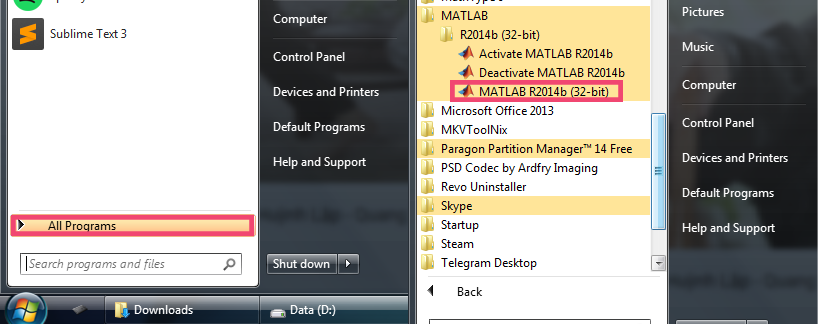
\includegraphics[scale=.7]{hinhtieuluan/pic1.png}
    \end{center}
    \caption{Thao tác mở chương trình từ Start Menu.}
    \label{refhinh1}
    \end{figure}
\end{center}
Giao diện chính của chương trình sau khi khởi động sẽ tương tự như hình bên dưới. Có 3 khu vực làm việc chính. Khung lớn nhất được bao viền màu xanh dương là Command Window. Khung Current Folder nằm ở phần trên, bên trái của Command Window. Phía dưới khung Current Folder là Khung Workspace.\\

\begin{center}
	\begin{figure}[htp]
	\begin{center}
		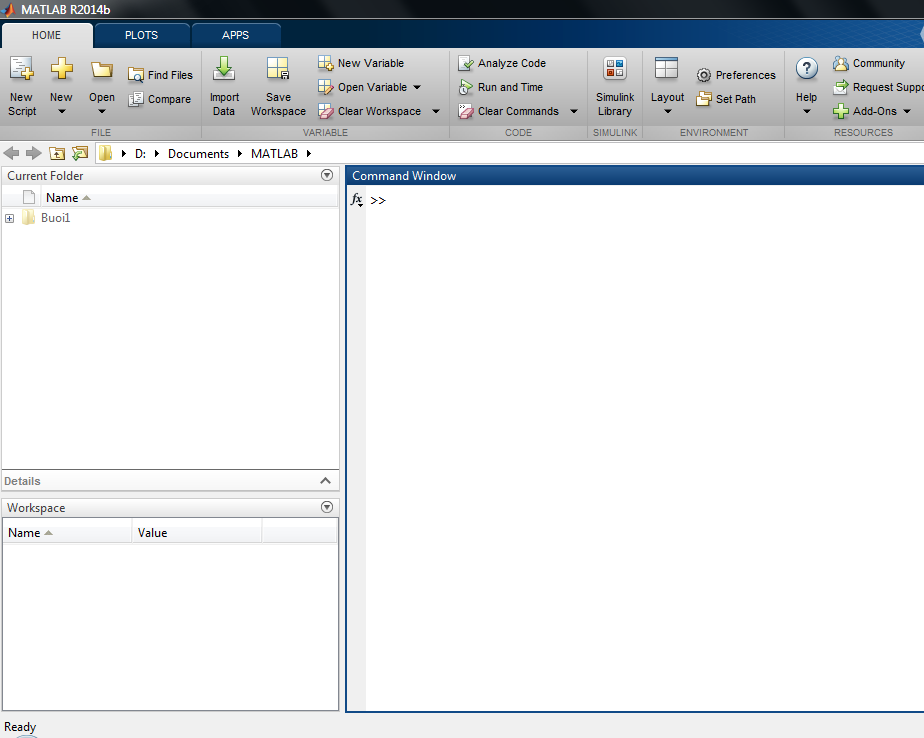
\includegraphics[scale=.6]{hinhtieuluan/pic2}
	\end{center}
		\caption{Giao diện chính của chương trình}
		\label{refhinh2}
	\end{figure}
\end{center}
Trong đó:\\
\begin{itemize}
	\item \textbf{Command Window:} Khu vực người dùng nhập các câu lệnh điều khiển và tính toán.
	\item \textbf{Current Folder:} Khu vực truy cập các tập tin m-file, m-hàm... được lưu trữ trên ổ đĩa máy tính.
	\item \textbf{Workspace:} Liệt kê các biến và dữ liệu đang được xử lý tạm thời. Ngoài ra người dùng có thể thao tác thêm bớt chỉnh sửa các giá trị của biến và tham số trực tiếp trên Workspace mà không cần dùng đến câu lệnh.
\end{itemize}
Ngoài ba khu vực chính trên, kể từ phiên bản MATLAB 2012a, thanh công cụ phía trên cùng truyền thống đã được thay thế bằng các thẻ lệnh Ribbon với biểu tượng cụ thể và rõ ràng hơn.\\
\begin{center}
	\begin{figure}[htp]
		\begin{center}
		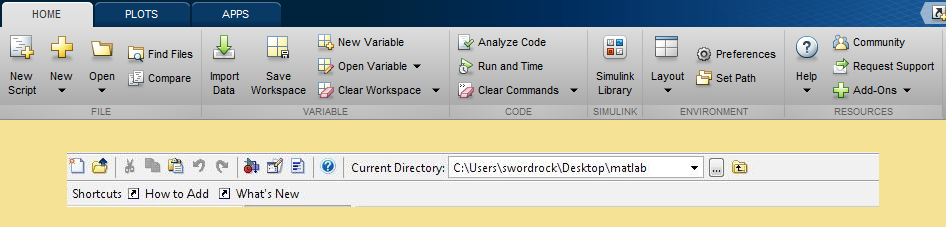
\includegraphics[scale=.5]{hinhtieuluan/pic3}
		\end{center}
		\caption{Thẻ Home (hình trên) ở giao diện mới và thanh công cụ truyền thống (hình dưới)}
		\label{refhinh3}
	\end{figure}
\end{center}
\subsubsection{Các thao tác cơ bản}
MATLAB thực hiện các phép cộng, trừ, nhân, chia như một chiếc máy tính bình thường. Xét các ví dụ đơn giản sau:\\
\textbf{Ví dụ 1:} Tính 3 + 2 + 6; 4 x 6 x 25 + 32 - 9 : 3.
\begin{lstlisting}
	>> 3 + 2 + 6 =
	ans=
				12
	>> 4 * 6 * 25 + 32 - 9 / 3 =
	ans=
				629
\end{lstlisting}
\textbf{Lưu ý:} MATLAB không quan tâm đến khoảng trắng giữa các dấu và luôn ưu tiên phép nhân rồi mới đến phép cộng. Kí hiệu \chuyencode{ans} là viết tắt của từ "answer" có nghĩa là kết quả của phép tính.\\
\textbf{Ví dụ 2:} Tính $sin{\dfrac{\pi}{2}}+cos{\dfrac{\pi}{2}}$\\
\begin{lstlisting}
	>>sin(\pi/2)+cos(\pi/2)=
	ans=
				1
\end{lstlisting}
Ngoài ra, người dùng có thể dùng lệnh \chuyencode{}
\subsection{Biến, câu giải thích, chấm câu}
\subsection{Các hằng số, các phép toán cơ bản, các hàm toán học}
\subsection{Quản lý tập, M-file, M-hàm}
%Chương 2:
\section{Các thao tác và phép toán với mảng}
%Chương 3:
\section{Vòng lặp điều khiển}
%Chương 4:
\section{Đồ thị trong mặt phẳng và trong không gian}
	%Bìa để sau
	
	%Mục lục
	
	Tiểu luận môn học Phần mềm Toán học

“Một số kiến thức về phần mềm MATLAB”

Chương 1: Cơ bản về MATLAB

1.1  Không gian làm việc

1.2  Biến, câu giải thích, chấm câu

1.3  Các hằng số, các phép toán cơ bản, các hàm toán học.

1.4  Quản lý tập, M-file, M-hàm

(C1 $\rightarrow$ C4)

Chương 2: Các thao tác và phép toán với mảng

(C6 và C7)

Chương 3: Vòng lặp điều khiển (C11)

Chương 4: Đồ thị trong mặt phẳng và trong không gian

(Bổ sung nhiều ví dụ và bài tập)
	%Test cho code
	\begin{lstlisting}
	// Hello.java
	for (i:1);
	import javax.swing.JApplet;
	import java.awt.Graphics;

	public class Hello extends JApplet {
    	public void paintComponent(Graphics g) {
        	g.drawString("Hello, world!", 65, 95);
    	}    
	}
	\end{lstlisting}
	
\end{document}